% !TEX TS-program = pdflatex
% !TEX encoding = UTF-8 Unicode
% arara: pdflatex: { draft: true }
% arara: biber
% arara: pdflatex: { synctex: true }
% arara: pdflatex: { synctex: true }

\documentclass[11pt]{article}

\usepackage[swedish]{babel} % Enables swedish typesetting, needs to be at top of document
\usepackage[T1]{fontenc}
\usepackage[utf8]{inputenc} % set input encoding (not needed with XeLaTeX
\usepackage{textcomp} % Suppress unicode char error
\usepackage{enumitem} % resume numbering in enumerations
\usepackage[bottom = 110pt]{geometry} % to change the page dimensions
%\geometry{a4paper} % paper format, could also be placed in documentclass options
\usepackage{graphicx} % support the \includegraphics command and options
\usepackage[parfill]{parskip} % Begin paragraphs with an empty line rather than an indent
\usepackage{verbatim} % adds environment for commenting out blocks of text & for better verbatim
%\usepackage{titling} % required for setlength droptitle (below)
%\setlength{\droptitle}{-70pt} % Adjust title height
\usepackage{fancyhdr} % This should be set AFTER setting up the page geometry
\pagestyle{fancy} % options: empty , plain , fancy
%\renewcommand{\headrulewidth}{0pt} % customise the layout...
%\lhead{}\chead{}\rhead{} % fancyhdr style reset for header
\usepackage{fancyvrb}
%\lfoot{}\cfoot{\thepage}\rfoot{} % fancyhdr style reset for footer
%\usepackage{sectsty} % Section title
\usepackage{hyperref} % href
\usepackage{caption}
\usepackage{subcaption}
\usepackage{nameref} % Enable referring to the actual name of the chapter
\usepackage[backend=biber,sorting=none]{biblatex}
\bibliography{references.bib}
\usepackage{url}

\title{Mobile-first eller Desktop-first, en studie om utvecklingslösningar för den responsiva webben}
\author{Eduardo Castaneda}
%\date{} % Uncomment to hide date, or provide a date to display


\pagestyle{fancy}               % Fräcka sidhuvuden
\addtolength{\headwidth}{0cm}   % Sidhuvd bredare än texten.
\renewcommand{\headrulewidth}{0.4pt}
\renewcommand{\footrulewidth}{0.4pt}

\begin{document}

\maketitle
\thispagestyle{empty}


\newpage

\begin{abstract}
Abstract goes here... Lorem ipsum dolor sit amet, consectetur adipiscing elit. Nam sollicitudin varius libero ac consectetur. Nullam ornare, massa et sagittis consectetur, neque mi scelerisque arcu, in fringilla lectus risus non arcu. Suspendisse vestibulum tellus id mauris lacinia non hendrerit nibh tempor. Proin tempor interdum justo et elementum. Ut ultricies adipiscing ipsum et pharetra. Vestibulum pretium luctus est, quis egestas augue luctus et. Praesent volutpat pharetra lectus vitae elementum.

Integer fringilla ligula eu sem semper tincidunt. Nullam mi lacus, blandit non sollicitudin eget, tempor eu ante. Cum sociis natoque penatibus et magnis dis parturient montes, nascetur ridiculus mus. Morbi ornare sem et purus consequat ac adipiscing nunc tincidunt. Curabitur nisi ante, ornare vel adipiscing et, scelerisque vitae erat. Etiam blandit egestas magna, quis dapibus nulla euismod quis. Sed interdum interdum malesuada. Suspendisse lacinia imperdiet laoreet. Maecenas ullamcorper laoreet nunc ac egestas. Cras consequat elit eu lacus sollicitudin ut pharetra magna venenatis. Suspendisse scelerisque condimentum pulvinar. Mauris ut tellus sit amet nulla porttitor tristique. Suspendisse eleifend erat sed nisi lacinia eu lacinia metus porta. Nulla pretium, risus eget semper laoreet, dolor odio malesuada eros, at mattis enim turpis gravida felis. Aliquam adipiscing varius nibh, ac auctor eros bibendum non.
\end{abstract}
\thispagestyle{empty}

\newpage
\tableofcontents

\newpage
\section{Bakgrund}

Mobilutvecklingen har under de senaste åren gått fort framåt, vilket har lett till att mobiler numera utvecklas till att fungera likt en handburen minidator. Huvudsyftet med mobiler är inte längre att bara kunna kommunicera med andra, utan även att bland annat ha möjligheten att få ut information genom webben. Att en websida inte längre endast ses i en skrivbordsskärm har gjort att nya webblösningar krävs. En utvecklare måste ha i åtanke att webbdesignen bör fungera för en användare som sitter på kontoret och läser sidan från en skrivbordsskärm, likaväl för en användare som sitter på tåget och läser sidan från mobilen. \textit{Responsive Web Design} är en lösning vilken beroende på skärmstorlek renderar samma sida på olika sätt. I responsive web design har det fokuserats på två olika metoder, \textit{Mobile-first} och \textit{Desktop-first}. Metoderna grundar sig på att utveckling sker för en typ av skärm först för att sedan utifrån det utveckla så att den sidan även passar för andra skärmar. Det finns mycket kunskap om metoderna var för sig, men inget underlag för valet av metod i olika situationer och inom olika områden. Mobilanvändarna ökar för varje dag medan skrivbordsanvändare behåller sina användare med en viss minskning. Det största antalet är användare utav båda, vilket kräver kunskap om när metoderna appliceras bäst för att få effektivare lösningar inom webutveckling.

\subsection{Mobilanvändare}

Sedan 2007 då Apple visade upp den första versionen av iPhone\cite{AppleRevolution} har utvecklingen för \textit{smartphones} eskalerat markant. Smartphones ger dig möjligheten att utföra datorliknande handlingar som att få ut information från webben och använda nätbaserade applikationer. Tidigare mobiler har delvis haft den funktionen men fokus mestadels har varit på musikspelare och kamera, då surfande gick trögt och var icke användarvänlig.
Med smartphones, vilket innebar större pekskärmar, gjorde åtkomsten till internet på mobilen mer användarvänlig och har under de senaste åren utvecklats till en oundviklig funktion i dagens mobiler \cite[s. 4]{Cfigroup_2009}.


Av svenskar mellan 12-79 år är det cirka 54 \% som använder sig av mobilt internet, i jämförelse med 2008 har det ökat med ungefär 70 \%. Under tidiga åren under 2000-talet låg ökningen per år på 1 \%, vilket visar att stora genombrottet har skett under de två senaste åren.\cite[s. 24]{.se}  Telefonoperatörer har anpassat sig till den nya marknaden och erbjuder abonnemanger vilka innehåller en fast kostnad för surf på ett 3G nät. Då mobilsurf anses som en nödvändig funktion, sätts krav hos mobiloperatörer i form av att hög åtkomlighet och en hög hastighet för 3G nätet\cite[s. 17]{Cfigroup_2009}. Effekten av att mobilanvändarnas åtkomst till internet ökar, leder till mobilt internet används mer och äldre tjänster ersätts. En tidning i tunnelbanan är inte alls lika vanlig nu som för fem år sen, tidtabell vid busshållplatsen är inte enda sättet att få ut information om busstider och att checka-in inför en flygresa behöver inte nödvändigtvis ske via en check-in disk\cite{kpcb}.

\newpage
Konkurrensen som finns i dagens mobilmarknad har tvingat ledande företag att skapa mobiler med ny teknik till allt lägre priser. Pris, tillgänglighet och användbarhet har gjort att användning av internet via mobilen i världen närmar sig antalet användare av internet via en dator\cite{morganstanley}. Analytiker som förutspådde mobilen till att slå i marknaden har i dagsläget fått det bekräftat och förutspår att användare av mobilt internet i världen kommer att passera antalet användare av Desktop internet  under år 2014\cite{morganstanley}. Detta kräver från webbplatser att följa målgruppen användare och anpassa webbsidor utifrån de enheter som webbsidor ses ifrån, vilket till stor del är från mobilen.

\subsection{Desktop användare}
Att mobilanvändare ökar för varje dag har till viss del ett samband med minskningen av antalet \textit{desktop} användare. Men datorer har i dagsläget funktioner som gör det osannolikt för mobiler att helt kunna ersätta datorer, funktioner som kräver att man sitter vid en dator och på så sätt sker informationssökandet i webben via desktop. 

Webbdesignen på en mobil är kompakt och uppfyller den nödvändigaste användbarheten.
På desktop är designen mer informationsrikt, vilket ger en större inblick till webbsidans innehåll och en mer simpel navigering på webbsidan. Det gör att en användare beroende på komplexitet och säkerhet av handlingen väljer att utföra den via en desktop \cite{userbeh}, än via mobilen. En sådan handling kan t.ex. vara bankärenden eller webshopping. Om bankärendet gäller en översikt av saldo i kontot eller överföring mellan egna konton, anses mobilen vara en smidig enhet att använda sig av. Däremot om handlingen innefattar att betala räkningar eller överföra stora summor pengar finns behovet av att utföra dessa handlingar via desktop, då det ger en större säkerhet och en mer simpel navigering på websidan. Även webshop faller i samma kategori, då användare väljer att söka information om produkten via mobilen, men väljer sedan att utföra köpet via desktop eller i affären\cite{userbeh}. Detta tyder på att användare av mobilt- eller desktop internet inte är endera, utan är användare utav båda, beroende på situation, miljö och kontext på webbsidan.

Det finns ingen grundlig faktum som tyder på att mobilt internet kommer att ta över all desktop internet användande, endast att de kan bli fler. Därför krävs det att man vidgar vyerna kring webutveckling och lösningar som gynnar både mobil- och desktop användning av internet. För även om mobila användare blir fler, så går det inte att förbise desktop användare.

\subsection{Responsive Web Design}

\textit{Responsive web design} är ett koncept som innebär att gränssnittet på en websida ändras beroende på skärmstorlek, vilket således ger möjligheten att ha olika layout på en och samma websida anpassat efter en enhet. Konceptet definierades av Ethan Marcotte (2010) i en artikel kallat \textit{A List Apart}, som sedan blev en del av boken \textit{”responsive web design”} där teorier och praktiska exempel används för att förklara begreppet. 

Syftet med Responsive Web Design är att kunna rendera olika delar av sidan beroende på skärmstorlek för att ge en optimal vy för den enhet webbsidan ses ifrån. Om tre element renderas bredvid varandra på en desktop sida, så vore det optimala för en mobilsida att kunna renderar elementen under varandra och även skala ner de till en rimlig storlek. På så sätt försvinner inte artiklarna från webläsarfönstret eller tar för stor plats på skärmen.

Då endast layouten på sidan ändras behövs inga särskilda versioner för varje enhet, vilket gör det möjligt för en webbutvecklare att på ett enkelt sätt utföra en ändring i en fil, istället för antalet versioner. Däremot krävs en flexibel grundlayout för att responsive web design skall fungera, vilket enligt Ethan görs genom tre grundtekniker, \textit{Fluid Grid}, \textit{Fluid Images} och \textit{Media Queries}\cite{resp}.

\subsubsection{Fluid Grid}
På en webbsida kan storleken på element definieras på olika sätt. Ett vanligt sätt att definiera element är med bredd och höjd i pixlar. När det definieras i pixlar betyder det att storleken på elementet är förutbestämd vare sig upplösning eller storlek på skärm. I tidigare skede informerade webbutvecklare användare vilken upplösning som renderade sidan på bästa sätt och sedan var upp till användaren att ändra upplösning på skärmen för att få den önskade layouten på sidan\cite[s. 6]{resp}. I dagsläget finns många olika skärmar, och många olika alternativ till upplösning vilket gör en förutbestämd storlek inte lika optimalt. 

Fluid Grid är en teknik vilken använder sig av procentsatser istället för pixlar vid definering av ett elements storlek. När procentsatser används förstoras eller förminskas elementets storlek relativt till webbläsarfönstrets höjd och bredd, vilket gör att sidan istället anpassas efter användaren. Om ett element skall täcka hela bredden på skärmen, sätts bredden till 100 \%, en fjärde del av skärmen, 25 \% osv. 
För att kunna bestämma elementets storlek i procentform härleder Ethan Marcotte ett sätt vilket innebär att, i pixelstorlek, dividera elementets storlek med behållarens storlek. Det ger ett resultat i procent, där elementet storlek ändras relativt till hållarens bredd och höjd \cite[s. 23]{resp}.

\subsubsection{Fluid Images}
Fluid Images bygger på samma princip som Fluid Grid, däremot är lösningen mer komplex då det innefattar skalning av bilder. Om en bild skalas på fel sätt leder detta till att bilden ser för utsträckt eller för intryckt ut, men om skalning inte görs, kan en bild i princip ta upp all plats på webbsidan och även försvinna ut i kanterna. Inom responsive web design används Fluid Images, vilket innebär en flexible hållare med en önskad storlek, med en bild anpassad till hållaren.  

Lösningen som tas upp av Ethan Marcotte är användningen av egenskapen "\textbf{max-width: 100 \%"} på bilden \cite[s. 45]{resp}. Med egenskapen "\textbf{"max-width:100 \%"}  talar man om för webbläsaren att bilden skall skalas efter hållaren men endast till max av den originella storleken på bilden. Egenskapen \textbf{”width:100\%”} innebär att bilden bara får anpassa sig helt efter hållaren, samtidigt som den får en normal skalning när storleken på webbläsaren minskar och hållaren krymper. Egenskapen \textbf{Max} i \textbf{”max-width”} innebär att bilden aldrig blir större än bildens verkliga storlek. Om \textit{”max”} inte sätts, finns risk att bilden skalas ut, vilket gör pixelkanter synliga. Däremot krävs det att man har en bild som redan från början är av önskad storlek. En för liten bild kommer den inte att förstoras då den som störst kan vara 100 \% av bildens ursprungliga storlek. Detta är ett sätt att ta använda sig av Fluid Images som fungerar för responsiva webbsidor, det kan uppstå andra komplikationer i form av att bilden inte skalas enligt önskemål där andra lösningar krävs, men grundtanken för att upprätthålla fluid images är att bilder skalas efter webbläsarfönstrets storlek.

\subsubsection{Media Queries}
Fluid Grid och Fluid Images skapar tillsammans en del av en responsiv sida då storleken på element i sidan renderas utifrån storleken på skärmen. Minskningen eller förstoringen av elementen fungerar däremot endast till en viss gräns. Vid tillfällen då storleken på webbläsaren för liten, finns risk att element kommer för nära varandra och skapar konflikt i layouten, det leder till att element hamnar på felaktiga positioner och ger en vy som designmässigt ser förstörd ut. Blir storleken däremot för stor, finns risk att \textit{max-width} på bilderna uppnås och stannar i storlek, medan andra element följer förstoringen hos webbläsaren, blir för stora och skapar en osymmetri i layouten. Media Queries är en lösning som tillåter element att ha olika värden beroende på skärmstorlek \cite[s. 65]{resp}.

Inom responsive web design är bredden och höjden viktiga egenskaper då de avgör hur mycket av en sida skall synas på webläsarfönstret.  Media queries är anrop som görs i CSS filen, där man kollar antingen höjden och eller bredden för att utföra nödvändiga ändringar i layouten för att upprätthålla en bra design. Tillsammans med Fluid Grid och Fluid Image skapar Media Queries en responsiv webbdesign. 

\newpage

Vid användning av fluid grid och fluid image sätts egenskaper hos element i procentform, t.ex 50 \%. Med en centrering på elementet, blir resultatet en ruta i mitten av skärmen som täcker 50 \% och har 25 \% utrymme på var sida. När webbläsarfönstret minskas till storleken av en mobilskärm anpassas elementet relativt till förändringen, då fluid grid tekniken används för bredden. Vilket ger oss dessa två vyer, ena med webbläsarfönstret i storlek av en skrivbordsskärm och den andra i storlek av en mobilskärm:

\vspace{0.5cm}
\begin{figure}[h]
\centerline{%
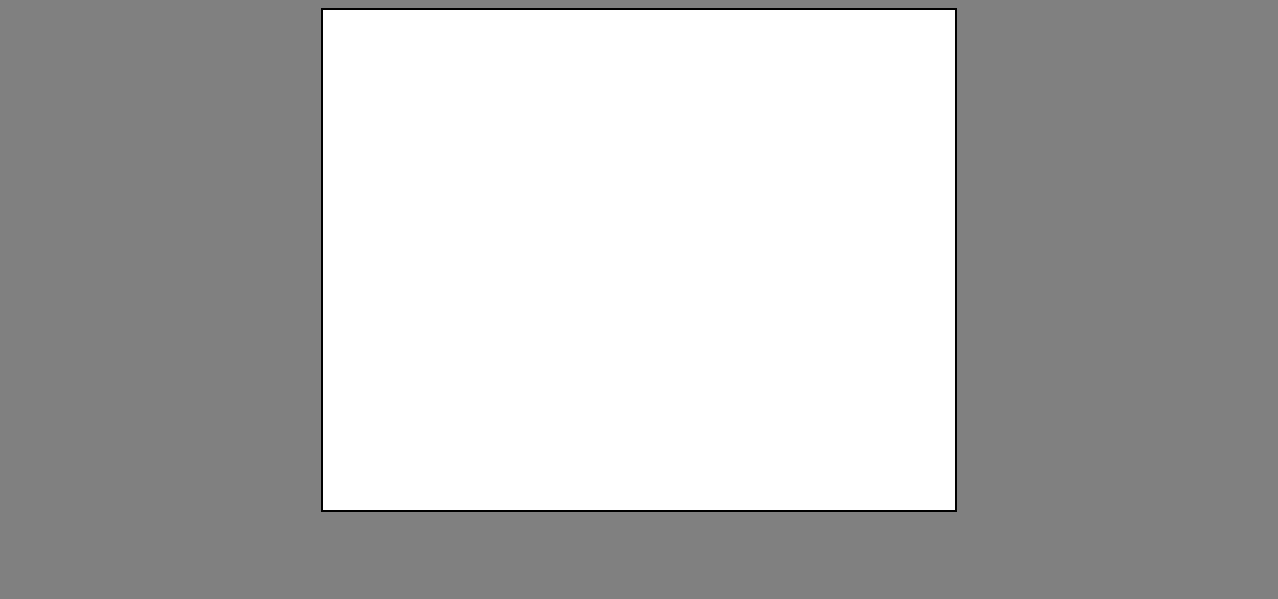
\includegraphics[scale=0.23]{pics/big.png}\hspace{5em}%
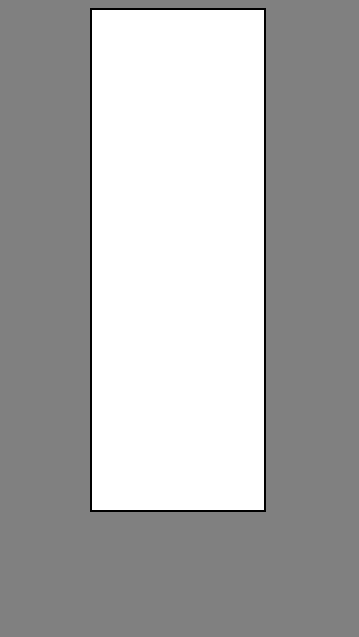
\includegraphics[scale=0.30]{pics/small.png}%
}
\end{figure}
\hspace{1.5cm}Figur 1: Utifrån desktop \hspace{4.8cm} Figur 2: Utifrån mobilen

\vspace{1cm}
Denna design har endast ett element med egenskaperna:

\vspace{0.5cm}
\begin{verbatim}

div {	
	        margin: 0 auto; //centrerad
	        width:50 %; //bredd
	        height:500px; //höjd
}

\end{verbatim}

Designen fungerar bra för skrivbordsskärmar\textit{(Figur 1)}, då rutan är centrerad och symmetrisk. 25 \% av utrymmet på var sida av rutan gör designen läsvänlig och användbart då fokusering sker i mitten av skärmen där förmodlingen information kommer att samlas. Däremot är den inte lika optimal när skärmen blir mindre\textit{(Figur 2)}. Rutan är fortfarande 50\% av skärmen, vilket gör att  designen blir kompakt i ett utrymme där förmedling av mycket information sker. 50\% procent av skärmen går till spillo åt utrymme mellan rutan och kanter, vilket får rutan att se ihoptryckt ut. Därav en försämring på design och användbarhet när webbsidan ses ifrån en mobilskärm.

Med media anrop i CSSen, kallat för media queries, tillåter vi att värden hos ”div” elementet skrivs över när bredden på webbläsaren underskrider 380px.

\vspace{0.5cm}
\begin{verbatim}
@media all and (max-width: 380px){
       div {
                margin:0;
                width:100%;
       }
}
\end{verbatim}
\vspace{0.5cm}

Med media anropet kommer \textit{”width”} och \textit{”margin”} skrivas över när skärmstorleken är 380px eller mindre, \textit{”height”} förblir detsamma. Utrymmet mellan kanterna och rutan ändras till "0" och bredden till "100 \%", vilket innebär hela skärmbredden. Detta leder till att sidan får andra designvärden när den ses från en mobil och andra enheter där skärmen har som störst 380px i bredd. Det ger en mer optimal lösning i både användbarhets och design perspektiv, då mer plats ges åt information och gör navigeringen lättare för en användare. 
\vspace{1cm}
\begin{figure}[h]
\centerline{%

\includegraphics[scale=0.25]{pics/mobilesmall.png}
}
\end{figure}
\centerline{Figur 3: Resultatet vid användning av media queries}
\vspace{0.5cm}

På så sätt kan samma CSS-fil låta element ha olika värden på egenskaper beroende på webbläsarstorlek. Responsive web design fyller sin funktion genom att tillföra en användbar design oavsett enhet som används för att se webbsidan. 
\newpage
\subsection{Verktyg}

Inom webdesignsutveckling används främst verktygen HTML, CSS och javascript, vilket är det verktyg som kommer att användas under implementeringsfasen i examensarbetet.  I kommande sektion av rapporten kommer verktygen att förklaras för att få en bättre förståelse till kod och termer som används.

\subsubsection{HTML}
HTML står för \textit{Hypertext Markup Language} och är ett format som definierar strukturen och logiken på en webbsida. HTML beskriver strukturen genom att märka upp olika delar av sidan med hjälp av \textit{taggar} som beskriver typen av ett element. En webbläsare läser av HTML-koden och kan på så sätt rendera sidan med önskvärd layout.

Det finns olika sorters taggar inom HTML, stycke, rubrik, tabeller, länkar, listor, sektioner är en av dessa. Inom webbutveckling har användning utav taggen \textit{<div>} blivit vanlig för att strukturera upp en sida i olika sektioner\cite{divtable}, vartefter kan en sektion innehålla andra element.

\vspace{1cm}
\begin{verbatim}
<div> 
          <h1> Mobile-first eller Desktop-first?</h1>
          <p>Frågan en webutvecklare ställer sig inför skapandet av
           en responsiv websida
          </p>
</div>
\end{verbatim}
\vspace{1cm}

I ovanstående HTML-kod har vi definierat en sektion på webbsidan med \textit{<div>} taggen, inom den sektionen har vi en rubrik som definieras med taggen \textit{<h1>} och ett stycke som definieras med taggen \textit{<p>}. Taggarna i html-koden bildar tillsammans strukturen på sidan, däremot så har inte html-koden någon kontroll över utseendet för taggarna, det sköts utav CSS.  

\subsubsection{CSS}
CSS står för \textit{Cascading Style Sheets} och är ett språk som beskriver utseendet på en webbsida.
Med hjälp av CSS-kod kan olika element i html-koden få ett speciellt utseende i form av storlek, färg och position. Det finns olika sätt att definiera css, man kan definiera det direkt i taggen t.ex \textit{<p style=”color:blue; width:50px”>Frågan en webbutvecklare ställer sig inför skapandet av en responsiv webbsida</p>} vilket kallas för \textit{inline-styling}. Man kan även i html filen, definiera utseendet i \textit{<head>} taggen, vilket kallas för \textit{internal styling}\cite{css}:

\vspace{0.5cm}
\begin{verbatim}
<head>
           <style>
           p {
           color:blue;
           width:50px;
           }
           </style>
</head>
\end{verbatim}
\vspace{0.5cm}

På så sätt får alla \textit{<p>} taggar i html-koden egenskaperna som sätts. Trejde sättet är att definiera det i en egen css-fil och länka till det från \textit{<head>} taggen i html-koden, vilket är det vanligaste av de tre sätten och kallas för \textit{external styling}. 
\vspace{0.3cm}
\begin{verbatim}
<link rel="stylesheet" type="text/css" href="main.css">
\end{verbatim}
\vspace{0.5cm}

I css-kod definieras utseendet av olika taggar. Det finns möjlighet att definiera samma tagg med olika utseenden, detta görs genom att sätta \textit{Klasser} och \textit{IDs} för varje element. Ett element kan ha olika klasser eller ids, vilket definieras med ett utseende i css-koden. Det gör att varje tagg som delar klassen, delar även utseendet:

\vspace{0.3cm}
I html filen:

\begin{verbatim}
<div id=”main-container”>
          <p class=”paragraf”>Mobile-first vs Desktop-first</p>
</div>
\end{verbatim}
\vspace{0.5cm}
I css filen:

\begin{verbatim}
#main-container {
        width:50%;
        background-color:grey;
}

.paragraf{
        font-size: 125%;
        color:black;
}
\end{verbatim}
\vspace{1cm}

I ovanstående kod kommer sektionen få utseendet som definieras som ID: \textit{main} i css-koden och paragrafen utseendet som definieras som Klass: \textit{paragraf}.


Dessa tre olika sätt att definiera utseendet visas enligt prioritering, inline-styling kod först, sedan internal och sist external. Anledningen till att external väljs främst är för att utseendet inte behövs definieras flera gånger, allt är samlat i en fil och det går snabbare att ladda sidans utseende\cite{css}. Därmed hålls det ur en webbutvecklares synvinkel, en bra struktur. Vilket tillåter webbutvecklaren att på upprätthålla teknikerna fluid grid, fluid images och på ett enkelt sätt använda sig av media queries vid implementering av en webbsida.

\subsubsection{JavaScript}
\textit{JavaScript} är ett scriptspråk som inom webbutveckling främst används för att hantera dynamiska funktioner för beteendet hos en websida, beteenden som skapas från klientsidan. Med JavaScript kan man t.ex. läsa en användarens klick i webbsidan och utifrån det kalla på funktioner som kan ändra webbsidans innehåll eller utseende. Eftersom JavaScript är ett skriptspråk behövs ingen kompilering och koden kan skrivas direkt i html-filen.

För att JavaScript skall fungera korrekt krävs det dock att webbläsaren stödjer det. I vissa fall har webbläsaren den funktionen men har den avstängd\cite[s.13]{sara_ingmar}. Tidigare ett problem varit att mobilwebbläsare inte har haft stöd för JavaScript, vilket har lett till att menyer och pop-up fönster inte har fungerat korrekt när man surfar till sidan via mobilen, men tekniken har utvecklats och numera klarar mobila webbläsare av JavaScript. Det finns fortfarande en del problem när det kommer till mer komplicerade JavaScript funktioner och bibliotek som mobilwebbläsare inte kan hantera\cite{quirksmode}. Vid webbsidor som har helt separata mobilsidor kan det vara en fördel då man väljer att inte läsa in all JavaScript som behövs, med responsiva webbsidor använder man samma webbsida för varje enhet, vilket leder till att en mobilenhet laddar all JavaScript vilket försämra webbsidans respons. En webbutvecklare måste ha i åtanke och redan från början utveckla en hemsida vars JavaScript inte kommer i vägen för den responsiva webbsidans funktionalitet.

\subsection{Mobile-first och Desktop-first}
Tekniken för att skapa responsiva webbsidor existerar, med hjälp av utvecklingen av ovanstående tekniker och verktyg finns i nuläget möjligheten att skapa webbsidor som beroende på skärmstorlek har olika designlayouts med en och samma kodgrund. Det finns även kunskap om hur man skall gå tillväga för att skapa en responsiv webbsida, där utvecklare med formler och riktlinjer kan lära sig att använda fluid grid, fluid images och media queries på bästa sätt. Men vägen till att skapa en responsiv websida är olika.  I bloggar och forum på webben diskuteras flitigt valet av utvecklingsmetod när det kommer till responsiva webplatser och innan implementeringen av en webbsida är detta en fråga som med stor sannolikhet dyker upp hos webbutvecklare. Utvecklingsmetoderna man diskuterar om är \textit{Mobile-first} och \textit{Desktop-first}. Mobile-first och Desktop-first är två olika metoder där det responsiva angreppssättet används. Båda strävar efter samma mål men skiljer sig i prioriteringen av vilken enhet webbsidan skall vara anpassad för först.

\subsubsection{Mobile-first}
Mobile-first metoden bygger på att man skapar en webbsida anpassad för mobilskärmen först, för att sedan med hjälp av media queries och en flexibel layout renderera elementen på webbsidan desto större webbläsarfönstret blir.  På så sätt är grund layouten designad för en mobil. Mobile-first anses som en rimlig utvecklingsmetod då man tar till hänsyn antalet mobilanvändare och det behov som finns vid navigering och informationsintagelse från mobilskärmar.  Det betyder att innehåll prioriteras då bristen på plats är ett faktum och fokus läggs på de delar som informationsmässigt är de viktigaste\cite{Mobilefirst}. Det behöver inte nödvändigtvis betyda att hänsyn till design för mobilen inte tas i desktop-first, utan snarare att implementationen för mobilskärm sker vid ett senare skede i utvecklingen än vid användning av mobile-first.

Kodmässigt är grunden anpassad för mobilen, det vill säga att media anrop sker när skärmen blir större, där media queries ser till att skriva om värden hos valda element. 
\vspace{0.5cm}
 \begin{verbatim}
@media all and (min-width: 480px){
        .main {
                margin:0 auto;
                width:50%;
        }
}
\end{verbatim}

\vspace{0.5cm}
I fallet ovan sker ett anrop när bredden på websidan är som minst 480px, som gör att elementen med klassen main får "\textit{margin"} och "\textit{width"} skrivs över med nya värden. I fall då mobiler inte klarar av att läsa media queries\cite{adaptiveresp}, vilket i dagsläget är få, är detta en optimal lösning då grunden redan är skrivet för mobilen och en läsning av media queries endast kommer att krävas från en skrivbordsskärm vilket de flesta webbläsare klarar av.

\subsubsection{Desktop-first}
Desktop-first metoden bygger på att man utvecklar för skrivbordskärmen först och därefter rendererar sidan desto mindre skärmen blir. Det behöver inte nödvändigtvis betyda att en färdig sida för desktop i efterhand designas om till mobil, utan tanken för mobil finns redan från början men implementeringen sker i synnerhet för skrivbordsskärmen först. Webbsidor som i efterhand skapas till mobilen, brukar innebära en separat mobilsida då refaktoreringen av kod i samband med att förvandla sidan till responsiv kan innebära en del komplikationer\cite{adaptiveresp}.  

Kodmässigt är grunden anpassad för skrivbordsskärmen. Det vill säga att media anrop sker när skärmbredden når en minimum gräns, där media queries ser till att skriva om värden på valda element.


\vspace{0.5cm}
 \begin{verbatim}
@media all and (min-width: 380px){
        .main {
                margin:0 ;
                width:100\%;
        }
}
\end{verbatim}
\vspace{0.5cm}

I fallet ovan sker ett anrop när bredden är som max 380px. Anropet ger "\textit{margin"} och "\textit{width"} i klassen main nya värden, anpassade till mobilen.  Desktop-first används oftast i samband med hemsidor där man vill skapa en upplevelse och vill att webbsidan skall nå ett design maximum när den ses utifrån en skrivbordskärm, upplevelsen utifrån en mobilskärm är inte lika högt prioriterad, men bör innebära en webbsida med den nödvändigaste funktionaliteten.

\subsubsection{Mobile-first eller Desktop-first, vilken skall man välja?}
Utvecklingen av tekniker och verktyg har gjort det möjligt att kunna applicera metoderna vid skapandet av en webbsida. Kunskapen om metoderna var för sig har med tiden blivit större i samband med utvecklingen av responsive web design. Däremot ställs webbutvecklare kring frågan om vilken metod som appliceras bäst till den typen av webbsida som skall skapas. I dagsläget finns ingen kunskap om hur bra metoderna appliceras i jämförelse med varandra. Det finns tankar och spekulationer, därefter väljs metod utifrån dessa, komplikationer hanteras men dokumenteras inte och till slut har man en fungerande responsiv webbsida. Eftersom webbsidan är färdig implementerad finns ingen anledning till att implementera om en fungerande lösning med en annan metod, därav finns ingen större kunskap om jämförelse av implementationen med respektive metod.

Användning av mobilt internet ökar och användningen av internet via en dator kommer med stor sannolikhet bestå. Vilket gör att en grund för val av metod är högst passande, då det redan nu och i framtiden kommer att kräva mer kunskap än vad som idag kan erbjudas från bloggar. Båda metoder har sina fördelar samt nackdelar, men frågan som bör ställas är när dessa går att utnyttjas på bästa sätt, och kan beslutet av val leda till positiva faktorer vilka motsatta metod inte hade kunnat uppnå inom en specifik situation.




\newpage

\section{Syfte}
Syftet med arbetet är att kunna hitta riktlinjer till när en specifik metod appliceras bäst. Det vill säga beroende på faktorer kring webbsidan hitta den metod som tillför det mest optimala lösningen för implementationen av webbsidan. Att hitta en metod som fungerar bäst i alla lägen är inte nödvändigtvis målet med arbetet då det existera många olika vinklar, vilka gör det svårt att hitta en specifik metod som ger det optimala resultatet oberoende på situation.

\vspace{0.5cm}
Frågeställningar som besvaras i rapporten är:
\begin{enumerate}
	\item I vilka lägen appliceras metoderna bäst?
	\item Vad är för- och nackdelarna med Mobile-first?
	\item Vad är för- och nackdelarna med Desktop-first?
\end{enumerate}
\vspace{0.5cm}
\textit{Frågeställning 1} baseras på miljö, målgrupp och kontext. Syftet med frågeställningen är att kunna utifrån analys hitta situationer där metoderna visar sig vara fördelaktiga under utvecklingsfasen, för att hitta faktorer hos metoden vilka motsatta metod inte har och därmed inte kan tillföra samma lyckade resultat. Syftet med \textit{Frågeställning 2 och 3} är att kunna lyfta fram de fördelar och nackdelar som finns vid implementation med de två metoderna. För att på så sätt hitta ramar för varje metod vilka en läsare kan relatera till med en egen situation och utifrån det använda det som grund vid val av metod. 

\subsection{Avgränsningar}

Arbetet kommer att enbart fokusera på mobile-first och desktop-first, ett mellanläge som existerar för Ipads, tablets, osv. kommer inte att tas med i arbetet. I dagsläget finns även andra lösningar för mobilt webb t.ex Appar och Hybrida Appar, jämförelse mellan dessa och responsive web design kommer inte att göras, utan jämförelsen som görs är mellan mobilalösningar inom responsive web design.

Termen \textit{Mobile-first} kan tolkas på olika sätt. Det har förekommit tillfällen för webbutvecklare där mobile-first är prioriterad designmässigt men där implementeringen ändå har skett för desktop innan mobilen, vilket en produktägare har tolkat som mobile-first. Det är inte fallet i arbetet, utan mobile-first beskrivs i arbetet som en tanke och en implementering avsedd för mobilen i första hand, och tvärtom vid desktop-first. Testfallen under implementeringsfasen i arbetet kommer att bygga på den teori för ovanstående metoder.

\newpage

\subsection{Valtech AB}
Examensarbetet kommer att utföras på Valtech AB i Stockholm. Valtech Sverige fokuserar främst på utveckling av användarvänliga hemsidor, webbapplikationer och intranät. Hos Valtech finns erfarna gränssnittsutvecklare som har stött på problem under utvecklingsprocessen i form av ett beslutstagande av tillvägagångssätt för en responsiv webbsida. Det finns ett behov hos utvecklare på Valtech att ha en grund för vilka faktorer som är viktigast vid beslutstagande för metod, en metod som ger den bästa lösningen för en effektiv utveckling av en responsiv webbplats. Gränsnittssutvecklarna besitter på mycket erfarenhet och kunskap, vilket kan samlas i form av intervjuer för att analyseras och sammanfattas utifrån verkliga situationer som förekommer i företag, för framtida syfte.
\newpage

%\section{Metod}
%För att kunna svara på frågeställningarna är tillvägagångsättet uppdelat i en praktisk del och en teoretisk del. Syftet med uppdelning är att kunna sammanställa resultat och diskussion med den erfarenhet som finns hos gränssnittsutvecklare genom en litteraturstudie, samt erfarenheten som fås utav den praktiska delen, i detta fall en implementering av båda metoder gentemot samma webbsida. Den praktiska delen vilket innebär gränssnittsutveckling, är den som tar mest tid och är den del som kommer att väga tyngst i arbetet. Litteraturstudien kommer att användas för att besvara det områden som resultatet av implementationen inte kan nå fram till, samt försvara de påståenden som fås utav implementationsfasen. 

%\subsection{Litteraturstudie}

%Litteraturstudien har utförts för att kunna samla de artiklar och punkter som är relevanta till metodernas applicering beroende på en webbsidas miljö, riktning av målgrupp och kontext. Men även för att kunna analysera användningen av mobilsurfande gentemot desktopsurfande. En analys av användningsområde för enheterna har kommit till användning vid val av prototyp för webbsidan som skall implementeras med de två metoder, samt för att stärka påståenden som har gjorts under implementationsfasen av examensarbetet. I Litteraturstudien har 3-5 artiklar angående användnings av mobilt- och desktop internet analyserats med avseende till webbsidans miljö, riktning av målgrupp och kontext. Användningen av enhet för webbsidor är en prioriteringsfråga som tas upp innan implementering, vilket kan vara den avgörande faktorn till val av metod. 

%\subsubsection{Miljö}
%Miljön baseras utifrån det område användningen utav webbsidan sker. Med det menas utifrån vilka sammanhang webbsidan kommer att besökas ifrån i första hand. T.ex. om det är en webbsida där miljön är kontor eller en webbsida där miljön resande, i vilka olika miljöer appliceras metoderna bäst? 

%\subsubsection{Målgrupp}

%I dagens läge är internet surfandet utspritt i många olika åldrar, vilket även gör målgrupp till en viktig faktor då användningen av enheterna existerar olika mycket bland olika åldrar. Det spelar en betydelsefull roll till det enhet vars webbsida kommer att ses ifrån och därmed kunna vara en prioriteringsfråga där olika implementeringsmetoder kan vara optimala för webbsidan beroende på målgruppen den är avsedd för.

%\subsubsection{Kontext}
%kontextet är sista faktorn som kommer vara en del av analysen, då kontext kan vara en avgörande faktor till val av layout. Valet av layout kan vara avgörande till enhet som bör prioriteras, då det finns en viss information som vill förmedlas till användaren som antingen kräver en större yta eller räcker med den yta som kan ges ifrån en mobilskärm.

%\subsection{Implementationk}
%Den praktiska och tekniska delen av examensarbetet utgörs utav en implementation av webbsida som både skall konstrueras i Mobile-first och Desktop-first. Syftet med implementationen är att jämföra vardera av metoderna genom att applicera dem för en och samma webbsida m.a.o. nå samma mål och resultat med två olika lösningar. För ha något att implementera har en prototyp designats och ritats utifrån det ramar som anses rimliga för att webbsidan skall spegla ett riktigt gränssnittsprojekt och även en hemsida vars besökare är både via mobilen och via desktop. Sedan har utifrån design för mobil och desktop, en webbsida i mobile-first och en webbsida i desktop-first skapats med hjälp av HTML-, CSS- och javascriptskod för att uppnå den gränssnittsfunktionalitet som eftersträvas, i det här fallet en responsiv webbsida. Under implementationens gång har en daglig rapport skrivits för varje metod. För att på så sätt kunna jämföra data gentemot samma period av implementeringsfasen för vardera av metoderna. Under implementationsfasen har komplexitet, total tid, kodstorlek och antal refaktoreringar använts som data för att jämföras.  Data för komplexitet har tagits ut genom rapporterna, med analys och en tidsmässig jämförelse på de problem som har dykt upp och lösningar för problemen. Under implementeringsfasen har lika mycket tid varit uppdelat per dag så att omständigheterna är detsamma för vardera implementation, vilket gör det möjligt att jämföra tiden med nogrannhet. Koden jämfördes i storlek i form av antal kodrader och filstorlek, samt en jämförelse lösningar där koden har skiljt sig. Refaktoreringar beskrivs som en ändring på någonting som redan funkar men som måste ändras på grund av att kommande implementeringar också skall funka som det ska. 

%\subsubsection{Prototyp}
%Prototypen är det första momentet i den praktiska delen. Rent designmässigt handlar det om att hitta en bra struktur på webbsidan så att den kan spegla ett verkligt gränssnittsprojekt där webbsidan uppfyller sitt syfte. Kontexten på webbsidan som skall implementeras har bestämts med hjälp utav en litteraturstudie där syftet är att hitta en typ av webbsida där besökarna är både mobilanvändare och desktop användare, vilket således är en svår situation för en gränssnittsutvecklare att bestämma implementeringsmetod. Därför krävs det av ritningarna att de uppfyller de nödvändigaste kraven i form av struktur och design.
%När sidtypen valdes ut, jämfördes den med andra webbsidor av samma typ och ritades ut med photoshop. Ritningarna avser en hel webbsida, mer än vad skärmen visar för att få en helhetsbild. Vid fall där menyer öppnas och stängs har ritningarna gjorts för vardera av fallen. Ritningarna har efter granskning, fastställts att gränssnittet skall kodas efter desas.
  
%\subsubsection{Dekstop-first}
%Prototypen är det första momentet i den praktiska delen. Rent designmässigt handlar det om att hitta en bra struktur på webbsidan så att den kan spegla ett verkligt gränssnittsprojekt där webbsidan uppfyller sitt syfte. Kontexten på webbsidan som skall implementeras har bestämts med hjälp utav en litteraturstudie där syftet är att hitta en typ av webbsida där besökarna är både mobilanvändare och desktop användare, vilket således är en svår situation för en gränssnittsutvecklare att bestämma implementeringsmetod. Därför krävs det av ritningarna att de uppfyller de nödvändigaste kraven i form av struktur och design.
%När sidtypen valdes ut, jämfördes den med andra webbsidor av samma typ och ritades ut med photoshop. Ritningarna avser en hel webbsida, mer än vad skärmen visar för att få en helhetsbild. Vid fall där menyer öppnas och stängs har ritningarna gjorts för vardera av fallen. Ritningarna har efter granskning, fastställts att gränssnittet skall kodas efter desas.  

%\subsubsection{Mobile-first}
%Mobile-first är andra implementeringsmetoden och utvecklades direkt efter desktop-first, då analysen av implementeringsfasen gjordes efter att båda rapporterna av utföranderna hade gjorts klar. Under implementeringen utvecklas även här webbsidan responsivt fråp början i form av fluid grids och fluid images. När webbsidan är klar för mobilen, påbörjas utvecklingen med media queries för att få en desktopvy utav de element som har utvecklats för mobilvyn. 

\printbibliography

\end{document}



